% !TEX root = ../thesis.tex
\chapter{Automatické rozpoznávání řeči}
\label{chap:asr}

Úlohou systému automatického rozpoznávání řeči (ASR) je převedení mluvené řeči na posloupnost slov, které řečník vyslovil. První takovéto systémy se začali objevovat v první polovine 20. století. První systémy pracovali na základě analýzy akustického signálu a porovnávání se vzorem. Byly tak schopny rozpoznávat jen velmi omezené množství slov. Významný zlom nastal v polovině 80. let minulého století, kdy se začali používat systémy založené na statistickém přístupu, konkrétně na HMM \cite{Holmes2001}. Pricipiálně je tento systém znázorněn on obr. \ref{fig:asr:decoding}. Řečový signál je analyzován a pomocí parametrizace převeden na sekvenci vektorů pozorování $O = \left\{o_1\ o_2\ \dots\ o_T\right\}$. Tyto vektory jsou u většiny systémů získávány s periodou $10\ ms$ pro segmenty řeči mající nejčastěji délku $20$ až $40\ ms$. Vlastní rozpoznávání pak probíhá v dekodéru, kde se systém snaží vybrat k vektorům pozorování $O$ takovou posloupnost slov $W = \left\{w_1\ w_2\ \dots\ w_N\right\}$, která maximalizuje aposteriorní pravděpodobnost (MAP)

\begin{equation}
  \hat{W} = \argmax_W\ P\left(W | O\right).
  \label{eq:asr:decoding}
\end{equation}

Pomocí Bayesova pravidla je možné podmíněnou pravděpodobnost $P\left(W | O\right)$ přepsat do tvaru

\begin{equation}
  P\left(W | O\right) = \frac{p(O|W)P(W)}{p(O)}.
\end{equation}

Jelikož pravděpodobnost $P(O)$ je z principu nezávislá na sekvenci slov $W$, je možné rovnici (\ref{eq:asr:decoding}) upravit do tvaru

\begin{equation}
  \hat{W} = \argmax_W\ p\left(O | W\right)P(W).
  \label{eq:asr:decoding:generic}
\end{equation}

Takto upravená rovnice představuje obecné pravidlo dekódování a její členy pak základní stavební prvky ASR systému. Podmíněná pravděpodobnost $p(O | W)$ odhaduje sekvenci pozorování $O$ na předpokladu slov $W$, tento výpočet je realizován \textbf{akustický model} (viz obr. \ref{fig:asr:decoding}). K vurčení $\hat{W}$ je ještě nezbytné mít pravděpodobnost výskytu požadované poslovnosti slov $P((W))$, o určení této pravděpodobnosti se stará \textbf{jazykový model}. Pro doplnění je nutné dodat, že \textbf{slovník} obsahuje seznam všech slov, se kterými je systém schopen pracovat. Tento seznam je všetně fonetické transkripce. Všechny tyto části jsou uvnitř \textbf{dekodéru}, který realizuje prohledávací strategii.

\begin{figure}[hbpt]
  \centering
  \includegraphics[width=0.9\textwidth]{./ch4-asr/img/decoding.pdf}
  \caption{Schéma automatického systému rozpoznávání řeči pracující na statistickém přístupu}
  \label{fig:asr:decoding}
\end{figure}

V následujícím textu jednotlivé stavební prvky ASR systému blížš popíšeme.

% !TEX root = ../thesis.tex
\section{Získání sekvence pozorování}
\label{chap:asr:parametrization}

Jako v mnoha jiných odvětvích, tak i při rozpoznávání řeči je v mnoha případech inspirací člověk. Pro získání sekvence pozorování (příznaků) vycházíme z \textbf{modelování produkce řeči} a \textbf{modelování procesu slyšení}, které se inspirují právě člověkem.

\subsubsection{Modelování produkce řeči}

Cílem modelování produkce řeči je nalezení matematických vztahů, které poslouží k reprezentaci fyzikálních dějů spojených s produkcí řeči. Základem je parametrizační technika \textbf{lineárního prediktivního kódování}, známá pod anglickou zkratkou LPC\footnote{Linear Predictive Coding} \cite{Benesty2007}. Vychází z představy, že hlasové ústrojí člověka je schopno vytvářet tři různé typy řečových zvuků:

\begin{itemize}
  \item \textit{samohlásky} - ty se řadí mezi znělé typy zvuků produkované periodickým buzením vznikajícím pulsy vzduchu, které jsou produkovány hlasivkami;
  \item \textit{frikativy} (např. $/f/$\footnote{Zápis $/f/$ symbolizuje foném, což je akustická reprezentace písmene, \textit{f}. Konkrétní zápisy se mohou lišit podle použité fonetické abecedy. V Čechách se nejčastěji používá abeceda $SAMPA$ či $Z\v{C}FA$.}) - někdy nazývané jako třené souhlásky, protože vznikají třením výdechovaného proudu vzduchu o překážku v některém místě hlasového ústrojí. Těmito překážkami může být jazyk, zuby ap.;
  \item \textit{explozivy} (např. $/b/$, $/p/$ ap.) - také nazývané jako souhlásky výbuchové, se tvoří úplnýn uzavřením vydechovaného proudu vzduchu pomocí artikulačních orgánů. To se následně projeví jako krázká pauza (tzv. okluze), po které následuje náhlé jednorázové uvolnění a únik nahromaděného vzduchu, tzv. exploze \cite{Psutka2006};
\end{itemize}

Snahou modelování je navržení modelu hlasového traktu, který bude dobře popisovat výše popsané zvuky. Nesmí se všask zapomenout na možnou složitost a přesnost modelu, jako ideální by byl linéárně časově invariantní model. Bohužel lidská řeč představuje kontinuální časově variantní a v některých situacích dokonce nelineární proces, takže je téměř nemožné jej přesně namodelovat. Pokud se včask udělají určité rozumné předpoklady, tak možné navrhnout lineární časově invariantní model řeči platný pro krátké časové úseky. Jinými slovy, předpokladem je, že v tomto krátkém časovém zůstává buzení a parametry hlasivkového traktu přibližně konstantní. Tento předpoklad přibližně platí pro intervaly $10$ až $30\ ms$. Odtud také vychází uvažovaná perioda segmntů řeči, viz úvod této kapitoly. Za těchto okolností je možné proces vytváření řeči modelovat pomocí tzv. \textbf{krátkodobého modelu}, který má v krátkých časových intervalech pevné parametry \cite{Holmes2001}.

\begin{figure}[hbpt]
  \centering
  \includegraphics[width=0.9\textwidth]{./ch4-asr/img/speech_model.pdf}
  \caption{Blokové schéma modelu produkce řeči}
  \label{fig:asr:model:speech}
\end{figure}

Pro odvození obecného diskrétního modelu hlasovkového traktu se vychází ze zjednodušeného modelu produkce řeči (obr. \ref{fig:asr:model:speech}). Ten je tvořen modelem hlasivek, modelem hlasivkového traktu a modelem vyzařovaného zvuku, které jsou seriově řazeny. K odvození a popisu vlastností modelu se využívá výhod z-transformace \cite{Psutka2006}. Po zjednodušení je krátkodobý model produkce řeči aproximovat celopólovým modelem (filtrem) $H(z)$ ve tvaru

\begin{equation}
  H(z) = \frac{G}{1 + \sum_{i = 1}^{Q} a_{i} z^{-i}} = \frac{S(z)}{U(z)},
  \label{eq:asr:lpc:generic}
\end{equation}

\noindent kde $G$ představuje celkové zesílení, $Q$ je řád modelu odpovídající $2K + 1$ počtu formantů, které má model postihovat, $a_i$ jsou parametry modelu. Vstupem modelu je buzení $u(k)$ (viz obr. \ref{fig:asr:model:speech}), tedy pro znělé zvuky sled pulsů s periodou $T_0$\footnote{Prioda základního hlasivkového tónu.} a pro neznělé zvuky náhodný šum s plochým spektrem. V časové oblasti je pak diskrétní výstupní odezva při fixovaných parametrech hlasového traktu ($10 - 30\ ms$) dána konvolucí a buzení a impulzní odezvy krátkodobého modelu. Na základě toho je možné model upravit na tvar podle obr. \ref{fig:asr:model:speech:excitation}, kde je $u(k)$ buzení a $s(k)$ je výstupní signál s parametry hlasového ústrojí odpovídající $a_i$ celopólového modelu.

\begin{figure}[hbpt]
  \centering
  \includegraphics[width=0.9\textwidth]{./ch4-asr/img/speech_process.pdf}
  \caption{Blokové schéma upraveného modelu produkce řeči}
  \label{fig:asr:model:speech:excitation}
\end{figure}

K odhadu parametrů $a_i$ slouží \textbf{lineární prediktivní analýza}. Odhad probíhá přímo z krátkodobého řečového signálu. Přenosové vlastnosti krátkodobého modelu je možné popsat rovnicí (\ref{eq:asr:lpc:generic}). Myšlenka metody LPC staví na předpokladu, že vzorek $k$ řečového signálu je možné popsat lineární kombinací $Q$ předchozích bzorků a buzení $u(k)$, což lze zapsat úpravou vztahu (\ref{eq:asr:lpc:generic}) do tvaru

\begin{equation}
  s(k) = - \sum_{i = 1}^{Q} a_i s(k-1) + Gu(k).
\end{equation}

\noindent Z něj patrné, že LPC se snaží parametry modelu $a_i$ odhadnou a zesílení $G$ odhadnout pomocí známe reálně naměřené posloupnosti $s(k)$. K vyřešení se používá principu minimalizace kvadratické chyby krátkodobé energie signálu. Ta je v časové oblasti popsána vztahem

\begin{equation}
  E = \sum_{k} e^2(k) = \sum_{k} \left[ s(k) - s'(k)\right]^2 = \sum_{k} \left( s(k) + \sum_{i = 1}^{Q} a_i s(k-1) + Gu(k) \right),
\end{equation}

\noindent kde $s(k)$ jsou vzorky reálného řečového signálu a $s'(k)$ jsou ty predikováné LPC filtrem. K získání řešení krátkodobé chyby predikce $E$, pro konkrétní analyzovaný segment, je použita metoda nejmenších čtverců. K výpočtu konkrétních koeficientů modelu $a_i$ je možné použít rekurzivního Durbinova algoritmu \cite{Holmes2001}.

Další možností jak popsat hlasový trakt je pomocí \textbf{kepstrálních koeficientů lineární predikce}. Pokud rovnici (\ref{eq:asr:lpc:generic})logaritmujeme, vznikne vztah

\begin{equation}
  \log H(z) = \log \left( \frac{G}{A(z)} \right).
  \label{eq:asr:lpc:cepstrum}
\end{equation}

\noindent Člen $A(z)$ je polynomem proměnné $z^{-1}$ řádu $Q$, a pokud všechny jeho kořeny leží uvnitř jednotkové kružnice, tak lze aplikovat Taylorův rozvoj na vztah (\ref{eq:asr:lpc:cepstrum}) ve tvaru

\begin{equation}
  \log \left( \frac{G}{A(z)} \right) = c(0) + c(1)z^{-1} + \dots = \sum_{k=0}^{\infty} c(k)z^{-k},
  \label{eq:asr:lpc:cepstrum:taylor}
\end{equation}

\noindent kde $c(k)$ jsou tzv. kepstrální koeficienty LPC. K odstranění logaritmu je potřeba obě strany rovnice derivovat. Po úpravě je výsledný vztah

\begin{equation}
  - \sum_{i=1}^{Q} ia_iz^{-i} = \left( \sum_{k=0}^{\infty} kc(k)z^{-k} \right)\left( \sum_{i=0}^{Q} a_iz^{-i}\right).
  \label{eq:asr:lpc:cepstrum:deriv}
\end{equation}

\noindent Pokud se $a_i = 1$, pak je možné roznásobení rovnice (\ref{eq:asr:lpc:cepstrum:deriv}) a porovnání člený u stejných mocnin $z$ zapsat vztahy pro výpočet kepstrálních koeficientů LPC

\begin{align}
  \begin{split}
    c(1) &= -a_1, \\
    c(k) &=
    \begin{cases}
      - a_k - \sum_{i=1}^{k-1} \left(\frac{i}{k}\right) c(i) a_{k-1},  & \quad \text{pro } 2 \leq k \leq Q, \\
      - \sum_{i=1}^{Q} \left(\frac{k - i}{k}\right) c(k-i) a_i,  & \quad \text{pro } k = Q + 1, Q + 2, \dots \quad ,
    \end{cases}
  \end{split}
  \label{eq:asr:lpc:cepstrum:coef}
\end{align}

\noindent kde $k = 1, 2, \dots , Q^{*}$ a $Q^{*}$ je počet kepstrálních koeficientů a $Q^{*} \geq Q$.

Kepstrální koeficienty LPC jsou vztaženy ke spektrální obálce mikrosegmentu řeči odvozené LPC analýzou, tu je možné získat dosazením $e^{j\omega}$ za $z$ v rovnici (\ref{eq:asr:lpc:generic}). Pro uspokojivou reprezentaci se tradičně volí $Q = 7\ \text{až}\ 15$ v závislosti na spektrální šířce přenášeného pásma, požadované přesnosti aproximace apod. Z toho plyne, že pro popis mikrosegmentu řeči by mohl stačit příznakový vektor o $15$ koeficientech.

\subsubsection{Modelování procesu slyšení}

Medelování procesu slyšení usilují o kompenzaci nelineárního vnímání frekvencí lidským sluchem. Dále pak i o respektování maskování zvuků včetně tzv. kritických pásem slyšení, což je přirozená vlastnost lidského sluchu. Maskováním se rozumí jev, kdy vnímání jednoho zvuku je ovlivněno přítomností jiného zvuku. Jinými slovy lze říci, že přitomnost jednoho zvuku zvyšuje práh slyšitelnosti pro jiný zvuk. Ten buď zní současně nebo s určitým časovým odstupem. Tento jev je jakýsi \uv{psychologický filtr}, který ignoruje věškerý šum ležící mimo ourčité kriticé pásmo. Šířka takového kritického pásma je přitom závislá na frekvenci poslouchaného tónu.

Typickým příkladem metod modelující proces slyšení jsou \textbf{melovská kepstrální filtrace} a \textbf{perceptivní lineární prediktivní analýza}.

TBD

% !TEX root = ../thesis.tex
\section{Akustické modelování}
\label{chap:asr:acoustic}

Akustický model představuje v rovnici (\ref{eq:asr:decoding:generic}) podmíněnou pravděpodobnost $p(O|W)$. Úkolem akustického modelu je poskytnout co nejpřesnější odhad této pravděpodobnosti pro libovolnou posloupnost vektorů příznaků $O = \left\{o_1 o_2\ \dots\ o_T\right\}$. Velmi vhodným způsobem modelování řeči se ukázalo být využití tzv. \textbf{skrytých Markovových modelů (HMM)}. Ty vycházejí z principu vytváření řeči člověkem. V průběhu produkce řeči se hlasové ústrojí nachází vždy v krátkém časovém úseku nachází v jednom z konečného počtu konfiguracé. V tomto mikrosegmentu je pak hlasovým ústrojím generovám krátký signál, který zavisí na aktuální konfiguraci. Tento vyprodukovaný zvuk je metodami (popsanými v \ref{chap:asr:parametrization}) převeden na vektor příznaků $O$.

Skrytý Markovův model je model stochastického procesu. Na ten je možné nahlížet jako na pravděpodobnostní konečný automat, který v diskrétních časových okamžicích generuje náhodnou posloupnost vektorů příznaků $O = \left\{o_1 o_2\ \dots\ o_T\right\}$. Model v každém časovém kroku změní stav svůj $s_j$ podle předem daných pravděpodobností přechodu $a_{ij}$. Přechod ze stavu $s_i$ do stavu $s_j$ má za následek vygenerování výstupního vektoru pozorování $o_t$ a to podle rozdělení výstpní pravděpodobnosti $b_j\left(o_t\right)$ příslušné k tomuto stavu \cite{Psutka2006}.

Podmínění pravděpodobnost přechodu $a_{ij}$ určuje, s jakou pravděpodobností přechází model ze stavu $i$ v čase $t$, do stavu $j$ v čase $t+1$. Platí tedy

\begin{equation}
  a_{ij} = p\left(s\left(t+1\right)=s_j|s\left(t\right)=s_i\right),
  \label{eq:asr:acoustic:conditional}
\end{equation}

\noindent kde $s\left(t\right)$ je stav modelu v čase $t$. Další podmínkou je, že pro všechny stavy $i$, $i=1,2,\dots\,N$, platí

\begin{equation}
  \sum_{j=1}^{N} a_{ij} = 1.
  \label{eq:asr:acoustic:state:condition}
\end{equation}

\noindent Funkce rozdělení výstupní pravděpodobnosti $b_j\left(o_t\right)$ popisují rozdělení pravděpodobnosti pozorování $o_t$ produkovaného ve stavu $s_j$ v čase $t$. Pro tuto funkci platí

\begin{equation}
  b_j\left(o_t\right) = P\left(o_t|s\left(t\right)=s\right),
  \label{eq:asr:acoustic:state:output}
\end{equation}

\noindent kde $P$ značí pravděpodobnost, pro kterou u diskrétních rozdělení platí

\begin{equation}
  \sum_o b_j\left(o\right) = 1.
  \label{eq:asr:acoustic:state:output:condition:discrete}
\end{equation}

\noindent Pro spojité rozdělení pak alternativně

\begin{equation}
  \int_o b_j\left(o\right)do = 1.
  \label{eq:asr:acoustic:state:output:condition:continous}
\end{equation}

\noindent V obou případech to platí pro všechny stavy HMM, které mohou generovat výstupní vektor.

Rozdělení výstupní pravděpodobnosti musí být při modelování řečových zvuků dostatečně specifické, aby bylo možné od sebe oddělit různé zvuky, a zároveň dostatečně robustní, aby zahrnulo značnou variabilitu řečového signálu. Toto rozdělení je možné modelovat

\begin{itemize}
  \item spojitým normálním rozdělením se směsí hustotních funkcí,
  \item neuronovými sítěmi.
\end{itemize}

\subsection{Struktura skrytého Markovova modelu}
\label{chap:asr:acoustic:HMM}

Z pohledu rozpoznávání řeči se nejčastěji využívá tzv. levo-pravá struktura Markovova modelu. V průběhu let bylo testováno mnoho různých struktur HMM, např. modely s počtem stavů odvozených od průměrné délky slova pro nějž byl model konstruován, až po pevnou strukturu stavů pro každé slovo. Tyto modely sloužily hlavně pro rozpoznávání izolovaných úseků řeči, nejčastěji slov. V současnosti, kdy je většina systémů konstruovaných pro zpracování souvislé řeči a počet slov ve slovníku může přesahovat 1 milion slov, převažují modely odvozené od menších jednotek, než jsou slova. Takovými jednotkami mohou být například fonémy anebo specifičtější trifóny. Trifón je svým způsobem kontextově závislý foném, který bere v potaz svůj levý a pravý kontext, tj. levý a pravý sousední foném. Přepis slova do fonémově, resp. trifónové struktury, lze ukázat na příkladu izolovaného slova \uv{akcie}, které má přepis \uv{\texttt{sil a k c i j e sil}}, v trifónové podobě je pak zápis následující

\begin{verbatim}
  sil sil-a+k a-k+c k-c+i c-i+j i-j+e j-e+sil sil,
\end{verbatim}

\noindent kde \texttt{sil} má význam pauzy před, případně za vyslovenou promluvou slova \uv{akcie}.

Oproti slovním modelům, u fonémů (monofónů), resp. trifónů, bývá struktura relativně jednoduchá a často je vyjádřena $5$ stavovým modelem (znázorněn na obr. TBD). Jedná se o $5$ stavový levo-pravý Markovův model, jehož první a poslední stav jsou tzv. neemitující. Jejich primární úlohou je zřetězování jednotlivých HMM modelů trifónů (monofónů) do rozsáhlajších modelů, např. slov, vět ap. Při zřetězení se tyto neemitující stavy vypouštějí. Ostatní stavy modelu jsou emitující a vztahují se k nim odpovídající rozdělení pravděpodobnosti $b_j(.)$.

Pokod předpokládáme, že posloupnost slov $W$ je modelována zřetězeným skrytým Morkovovým modelem $\Theta$, kde dílčí modely odpovídají fonetickým jednotkám, pak je možné určit pravděpodobnost generování posloupnosti $O$ modelem $\Theta$ jako

\begin{equation}
  P\left(O|\Theta\right) = \sum_{\forall S} P\left(O, S| \Theta\right)P\left(S|\Theta\right) = \sum_{\forall S} a_{s\left(0\right)s\left(1\right)} \prod_{t=1}^{T} b_{s\left(t\right)}\left(o_t\right)a_{s\left(t\right)s\left(t+1\right)},
  \label{eq:asr:acoustic:structure:output}
\end{equation}

\subsection{Gausovké směsi}
\label{chap:asr:acoustic:GMM}

TBD

\subsection{Využití neuronových sítí}
\label{chap:asr:acoustic:DNN}

\begin{figure}[hbpt]
  \centering
  \includegraphics[width=0.7\textwidth]{./ch4-asr/img/neuron.pdf}
  \caption{Schéma perceptronu}
  \label{fig:asr:acoustic:neuron}
\end{figure}

\begin{figure}[hbpt]
  \centering
  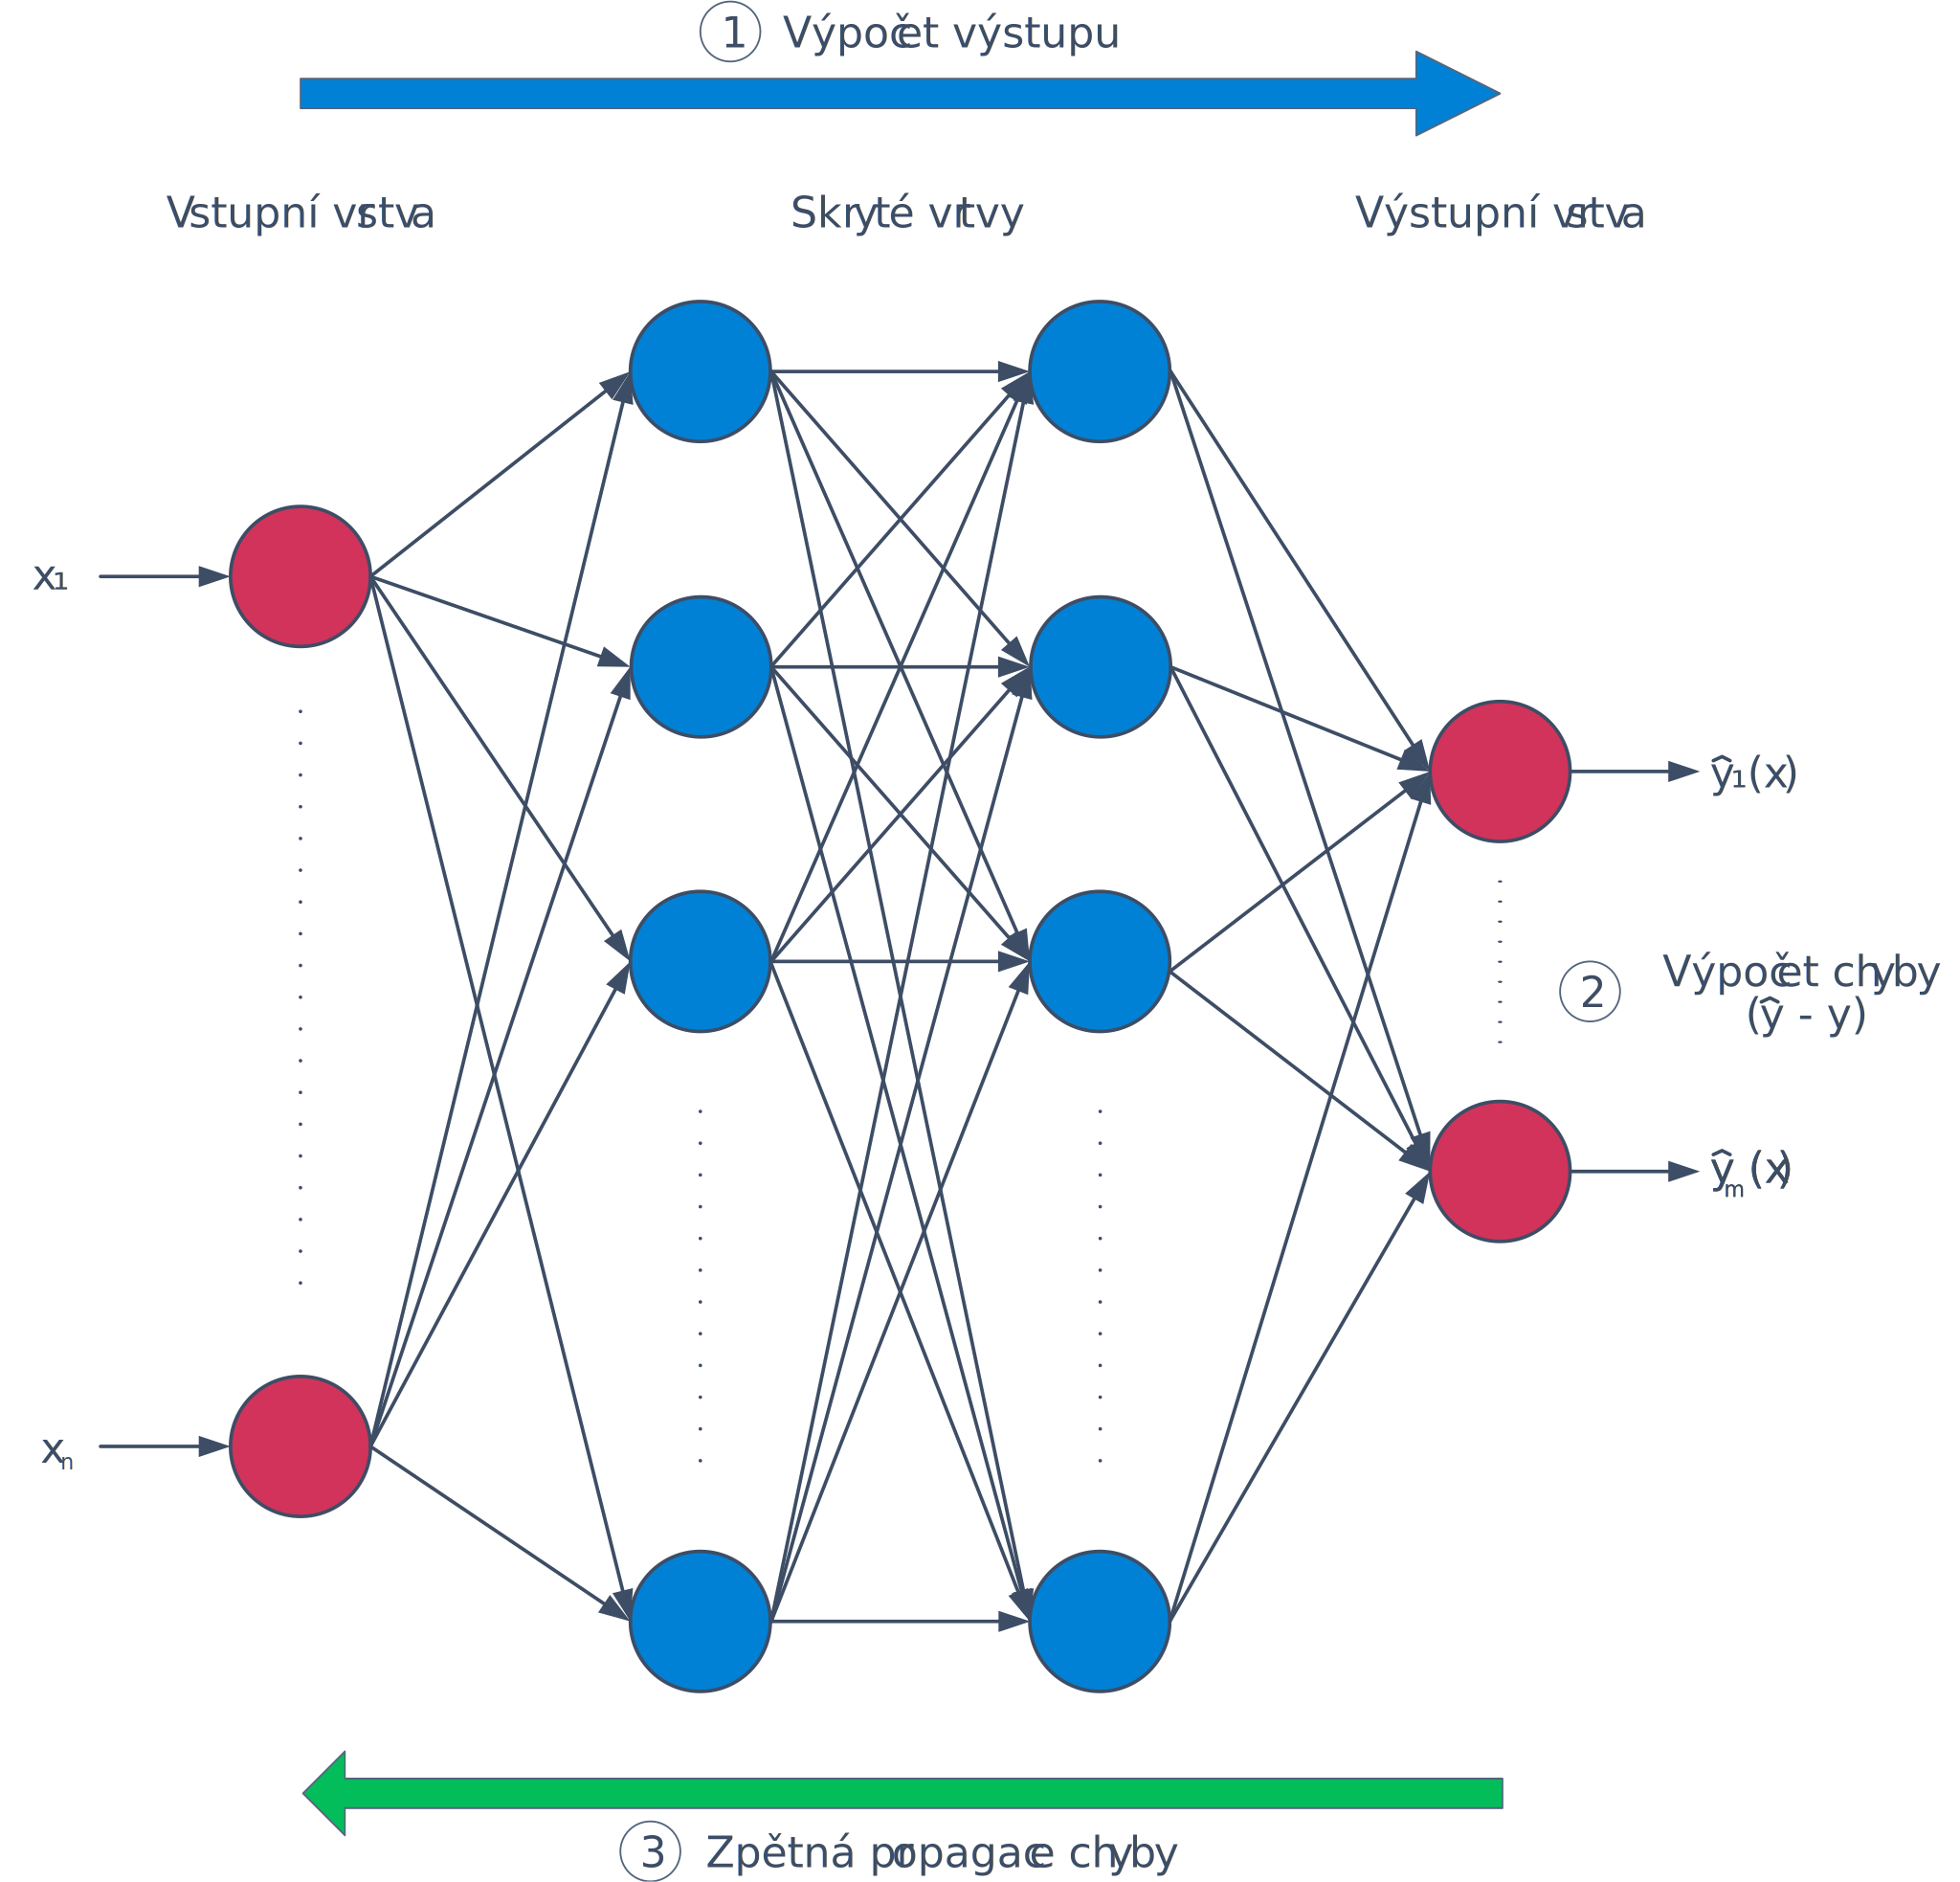
\includegraphics[width=0.9\textwidth]{./ch4-asr/img/dnn-training.pdf}
  \caption{Schéma a princip učení neuronové sítě}
  \label{fig:asr:acoustic:dnn}
\end{figure}

% !TEX root = ../thesis.tex
\section{Jazykové modelování}
\label{chap:asr:language}

TBD

% !TEX root = ../thesis.tex
\section{Dekódování}
\label{chap:asr:decoding}

Hlavní funkcí dekodéru je nalézt nejlepší výstupní posloupnost slov $\hat{W}$. Matematicky lze tento proces popsat pomocí vztahu

\begin{equation}
  \hat{W} = \argmax_{W} P\left(\boldsymbol{O} | W\right)P\left(W\right),
  \label{eq:asr:decoding:decoder}
\end{equation}

\noindent kde $P\left(\boldsymbol{O}|W\right)$ představuje již popsaný akustický model, $P\left(W\right)$ opisuje jazykový model. V~některých případech je úloha dekódování zobecněna na nalezení více než jedné posloupnosti slov $\hat{W}$. V~těchto případech se mluví jako o hledání \textbf{\textit{N} nejlepších} (\textit{N}-best) posloupností slov $\hat{W}$.  Řešení této úlohy je netriviální, protože dekodér obvykle nemá informaci o počtu slov v~dané promluvě, protože ASR systémy nevyžadují vyslovování pauz mezi jednotlivými slovy. Navíc, i kdyby tato informace byla  k~dispozici, tak pro promluvu, která čítá $M$ slov, je se slovníkem čítajícím $N$ slov, potřeba prozkoumat $N^{M}$ různých slovních kombinací (hypotéz), tj. například $10^{50}$ vyhodnocení při $N=100000$ a $M=10$. Z toho jasně plyne, že aplikace metody vyčerpávajícího prohledávání je i pro úlohu s~malými slovníky a krátkými promluvami nerealizovatelná.
Naštěstí bylo navrženo několik účinných algoritmů, které řeší úlohu hledání maxima (\ref{eq:asr:decoding}) bez exponenciálního nárůstu počtu výpočtů. Mezi takové algoritmy patří dekódování podle \textbf{kritéria maximální aposteriorní pravděpodobnosti (MAP)}, nebo v~současnosti primárně používaného dekódování podle \textbf{Viterbiova kritéria}.

Akustický model zjišťuje pravděpodobnost $P\left(\boldsymbol{O}|W\right)$, resp. $P\left(\boldsymbol{O}|\lambda\right)$ pomocí forward-backward (FB) algoritmu.
Ten pro pozorovanou posloupnost $\boldsymbol{O}$ určí pravděpodobnosti všech možných cest délky $T$ modelem $\lambda$.
Výpočet podmíněné pravděpodobnosti lze aproximovat pravděpodobností $P_S(\boldsymbol{O}|\lambda)$, reprezentující nejpravděpodobnější posloupnost HMM stavů, kterými projde posloupnost $\boldsymbol{O}$ modelem $\lambda$, tedy

\begin{equation}
  P\left(\boldsymbol{O}|\lambda\right) \approx P_S\left(\boldsymbol{O}|\lambda\right) = \max_S P\left(\boldsymbol{O}, S| \lambda \right) = \max_S a_{s\left(0\right)s\left(1\right)} \prod_{t=1}^{T} b_{s\left(t\right)}\left(\boldsymbol{o}_t\right) a_{s\left(t\right)s\left(t+1\right)}.
  \label{eq:asr:decoding:approx}
\end{equation}

\noindent Tuto pravděpodobnost i optimální posloupnost stavů lze určit tzv. \textbf{Viterbiovým algoritmem} \cite{Holmes2001}. Ten řeší úlohu s~využitím heuristického prohledávání typu beam. Protože vždy expanduje pouze několik nejslibnějších uzlů, dochází  k~urychlení výpočtů časově synchronního prohledávání, a tedy i  k~prořezávání neperspektivních hypotéz.

Pro další urychlení dekódování (zejména u systému pracujících v~reálném čase) bylo navrženo několik dalších sofistikovaných postupů, např. využití tzv. lexikálních stromů nebo jiných technik prořezávání, případně zjednodušení akustického modelu slova. Více o této problematice v~\cite{Psutka2006}.

U reálného systému je často potřeba vyřešit nebo \uv{vybalancovat} poměr příspěvků pravděpodobností od akustického a jazykového modelu. Z principu fungování ASR systémů vyplývá, že upřednostňují při dekódování krátká slova, což způsobuje chybu typu vložení. Ta se kompenzuje tzv. penaltou vložení, která mění měřítko $P(\boldsymbol{O}|W)$ a $P(W)$ v~závislosti na počtu slovních hypotéz. Jinými slovy penalizuje vložení krátkého slova v~případě, že se jako \uv{lepší} jeví delší slovo. Pro vyvážení příspěvku jazykového modelu se ve většině systémů používá tzv. \uv{grammar scale factor}. S využitím výše uvedených poznatků lze vztah (\ref{eq:asr:decoding:decoder}) určující odhad obsahu promluvy upravit do tvaru

\begin{equation}
  \hat{W} = \argmax_{W} \left[\log P\left(\boldsymbol{O}|W\right) + \kappa_1 \log\left(P\left(W\right) + \kappa_2H\right)\right],
  \label{eq:asr:decoding:compensated}
\end{equation}

\noindent kde $\kappa_1$ je faktor změny měřítka, $\kappa_2$ je penalta vložení a $H$ celkový počet obsažených slov v~hypotéze. Hodnoty parametrů $\kappa_1$ a $\kappa_2$ jsou většinou určovány experimentálně.

V úloze rozpoznávání spojité řeči se vyskytují 3 typy chyb:

\begin{itemize}
  \item \textit{substituce (S)} - došlo  k~rozpoznání špatného slova;
  \item \textit{deletace (D)} - došlo  k~vynechání nějakého slova;
  \item \textit{inzerce (I)} - došlo  k~vložení slova, které nebylo součástí promluvy $W$.
\end{itemize}

\noindent K evaluaci schopností systému rozpoznávání řeči se pak využívá vzorce pro výpočet míry chybovosti na slovech (WER)

\begin{equation}
  WER = \frac{C(S) + C(D) + C(I)}{N},
  \label{eq:asr:decoding:wer}
\end{equation}

\noindent kde $N$ představuje počet slov v~$\hat{W}$ a $C(.)$ je funkce určující celkový počet chyb konkrétního typu. Čím je hodnota $WER$ nižší, tím systém poskytuje přesnější odhad. Velmi často se také používá metrika přesnosti rozpoznání udávaná v~procentech. Stejně jako $WER$ je definována pomocí vyčíslených chyb systému. Matematicky lze tuto relaci zapsat pomocí vztahu

\begin{equation}
  Acc = \frac{N - C(S) - C(D) - C(I)}{N} * 100.
  \label{eq:asr:decoding:acc}
\end{equation}

\noindent Po úpravě výše uvedeného vztahu lze získat relaci mezi oběma metrikami, konkrétně $Acc = \left(1 - WER\right) * 100$. Z toho plyne, že oproti $WER$ je systém s~vyšší přesností lepší než systém s~nižší přesností.

% % !TEX root = ../thesis.tex
\section{Vyhodnocení}
\label{chap:asr:evaluation}

TBD


% Jedním z hlavních důsledků TL (popsané v \todo{TBD}{[xx]}) je ztráta hlasivek a tím i hlasu. Problematikou komunikace pomocí mluvené řeči i v situacích, kdy akustický řečový signál není k dispozici, se zabývají  systémy zpracovávající \uv{tichou} řeč (angl. Silent speech interface, zkr. SSI). Ve většině případů se snaží získat informaci, která je normálně zakódována v akustickém signálu získat jinou cestou.

% Produkce mluvené řeči je komplexní proces, který začíná v možku a končí produkcí slyšitelného zvuku. Pokud odstraníme komponentu starající se o vznik zvuku, ještě to neznamená, že i ostatní komponenty také ztrácejí svou funkci. Tento fakt je základní premisou pro funkci všech v současnosti vyvíjených SSI systémů.

% Vývoj komplexního SSI je velmi náročný problém, který se zatím (i přes nemalé usílí) doposud nepodařilo uspokojivě vyřešit.

% \begin{itemize}
%   \item lehce popsat technické přístupy
%   \begin{itemize}
%     \item NAM
%     \item magnety
%     \item brain interface
%   \end{itemize}
% \end{itemize}
